A homologia persistence teve seu ínicio em uma intersecção entre as ciências da computação 
e a matemática. Os primeiros artigos mostravam algoritmos sobre espaços topológicos simples,
como esferas \cite{Edelsbrunner2000}. No entanto, a teoria foi se desenvolvendo 
ao longo dos anos ao ponto em que as linguagens utilizadas para tratar da homologia persistente 
é a teoria de categorias conjuntamente com a teoria de representações \cite{Chazal2016}.

Neste capítulo tratamos do desenvolvimento da homologia persistente sob a luz dessas linguagens. 
Na primeira seção definimos o que são os módulos de persistência e suas relações com os diagramas de 
persistência. Na segunda seção descrevemos a medida retangular, usada para abstrair o conceito 
de diagrama de persistência e poder estudar o quão \textit{tame} ele o é. Apresentamos na terceira seção
alguns exemplos do comportamento dos módulos de persistência e exemplos. A quarta seção é fundamental,
pois mostramos como comparar dois módulos de persistência, através do \textit{interleaving}. E finalmente,
apresentamos o teoria de isometria e mostramos uma das implicações com a teoria desenvolvido neste capítulo. 

\section{Módulos de persistência e decomposições}
Nesta seção iremos definir os módulos de persistência, apresentar teoremas de decomposição dos módulos 
e introduzir a notação de quiver, que será utilizada para as próximas seções e demonstrações de 
outros resultados. 

Fixaremos aqui o corpo $\mathbf{k}$ para todos os espaços vetoriais apresentados neste texto. 

\begin{defi}
    Um módulo de persistência $\mathfrak{V}$ sobre os números reais $\mathbb{R}$ é uma família indexada 
    sobre $\mathbb{R}$ de espaços vetoriais 
    \begin{equation*}
        (V_t \mid t \in \mathbb{R}), 
    \end{equation*} 
    e uma família de aplicações lineares duplamente indexadas
    \begin{equation*}
        (v_t^s \colon V_s \to V_t \mid s \leq t) 
    \end{equation*}
    que satisfazem a seguinte relação de composição
    \begin{equation*}
        v_t^s \circ v_s^r = v_t^r,
    \end{equation*} 
    em que a função $v^r_r$ é considerada a função identidade. 
\end{defi}

O módulo de persistência pode ser visto como um funtor entre a categoria dos números reais com o morfismo
$s \to t$, em que $s \leq t$ e a categoria de espaços vetoriais. 

Vamos dar um exemplo de módulo de persistência que se encontra no contexto de análise topológica de dados. 
Seja $X$ um espaço vetorial e $f \colon X \to \mathbb{R}$ uma função, não necessariamente contínua e 
considere os conjuntos de nível
\begin{equation*}
    X^t = (X,f)^t = \Set{x \in X \mid f(x) \leq t}.
\end{equation*}

Temos uma sequência de conjuntos encaixados, $X^t$ com $t \in \mathbb{R}$, ou seja, existe uma função 
inclusão $\iota_t^s \colon X^s \hookrightarrow X^t$ que satisfaz trivialmente a lei de composição e 
existe uma função identidade. Chamamos esta sequência de conjuntos e funções de filtração de subníveis
de $(X,f)$, denotada por $\mathfrak{X}_{sub}$ ou $\mathfrak{X}^f_{sub}$.

Dada a sequência acima, podemos transforma-la em um módulo de persistência utilizando qualquer funtor
da categoria de espaços topológicos para a categoria de espaços vetoriais. Neste caso utilizamos 
o funtor de homologia $H = H_k(-, \mathbf{k})$ de dimensão $k$ com coeficientes em $\mathbf{k}$. Assim,
podemos definir o seguinte módulo de persistência $\mathfrak{V}$

\begin{equation*}
    V_t = H(X^t) \qquad v^s_t = H(\iota_t^s) \colon V_s \to V_t.
\end{equation*}
Podemos também escrever $\mathfrak{V} = H(\mathfrak{X}_{sub})$. 

Um exemplo na análise topológica de dados é quando $X$ é um complexo simmplicial finito e $X^t$ é um 
subcomplexo. Devido as propriedades dos complexos, existem finitos valores críticos onde há mudanças 
em $X$. Suponha que os valores sejam $a_1 < \dots < a_n$. Entao toda a informação do módulo de 
persistência é dada pela seguinte sequência de espaços vetoriais de dimensão finita

\begin{equation*}
    H(X^{a_1}) \to \dots \to H(X^{a_n}).
\end{equation*}

Neste caso, $H(\mathfrak{X}_{sub})$ admite uma descrição compacta, existe um algoritmo eficiente para 
o seu calculo e por último, a descrição é contínua com relação a $f$, ou seja, é estável sob uma 
métrica. 

A descrição mencionada acima é o diagrama de persistência ou barcode. A estrutura é dada por uma 
lista de intervalos da forma $[b,d) = [a_i, a_j)$ ou $[a_i, +\infty)$. Cada intervalo representa
um ciclo, uma propriedade, que nasce em $b$ e morre em $d$. 

Iremos mostrar aqui que é possível associar um diagram de persistência para módulos de 
persistência $\mathfrak{V}$ \textit{q-tame}. Um módulo de persistência é \textit{q-tame} 
se 
\begin{equation*}
    r_t^s = \text{rank}(v_t^s) < \infty \text{ para } s < t.
\end{equation*}
Intuitivamente falando, um módulo é \textit{q-tame} se para todo quadrante que pegamos com a origem
na diagonal, existem finitos pontos do diagram de persistência neste quadrante como pode ser visto
na \autoref{fig:quad_finito}.

\begin{figure}
    \centering
    
\includegraphics[width=0.5\textwidth]{images/placeholder.png}
    \caption{Exemplo de um diagram de persistência de um módulo de 
            persistência \textit{q-tame} com um quadrante em destaque.}
    \label{fig:quad_finito}
\end{figure}

\subsection{Indíces e posets} 
No início desta seção definimos o módulo de persistência com o conjunto de indíces sendo os reais. No 
entanto, é possível definir utilizando quaisquer conjuntos parcialmente ordenados da mesma forma que 
com os reais. Seja $\mathbf{T}$ um poset, a coleção de espaços vetoriais e aplicações lineares que 
satisfazem as leis de composição e identidade é chamada de $\mathbf{T}$-módulo de persistência, ou 
módulo de persistência sobre $\mathbf{T}$. 

Além disso, podemos restringir o poset $\mathbf{T}$ para um subconjunto $\mathbf{S} \subset \mathbf{T}$
de forma a obter o $\mathbf{S}$-módulo de persistência, que são os espaços vetoriais e aplicações lineares
cujos indíces são elementos de $\mathbf{S}$. Esta é a restrição de $\mathfrak{V}$ em $\mathbf{S}$ e pode
ser denotada por $\mathfrak{V}_S$ ou $\left.\mathfrak{V}\right|_S$. 

\subsection{Categoria de módulos}
Com a definição de módulos de persistência sobre um poset $\mathbf{T}$ qualquer, podemos definir
homomorfismos entre módulos. Sejam $\mathfrak{U}, \mathfrak{V}$ $\mathbf{T}$-módulos de persistência.
Um homomorfismo $\Phi$ entre $\mathfrak{U}$ e $\mathfrak{V}$ é uma família de aplicações lineares 
$(\phi_t \colon U_t \to V_t \mid t \in \mathbf{T})$ tal que o seguinte diagrama comuta para todo
$s \leq t$. 

\begin{equation*}
    \begin{tikzcd}
        U_s \arrow{d}[swap]{\phi_s} \arrow{r}{u_t^s} & U_t \arrow{d}{\phi_t} \\
        V_s \arrow{r}{v^s_t}                     & V_t                    
    \end{tikzcd} 
\end{equation*}

A composição de dois homomorfismo $\Phi, \Psi$ é dada por cada indíce $t \in \mathbf{T}$, ou seja,
$\Phi \circ \Psi$ é a coleção de aplicações lineares $(\phi_t \circ \psi_t \colon U_t \to W_t \mid t \in \mathbf{T})$,
onde $\Phi$ é homomorfismo entre $\mathfrak{U}$ e $\mathfrak{V}$ e $\Psi$ entre $\mathfrak{V}$ e $\mathfrak{W}$. 
A identidade é definida de forma trivial. Portanto, temos a categoria dos módulos. Definamos os seguintes conjuntos
\begin{align*}
    \text{Hom}(\mathfrak{U}, \mathfrak{V}) &= \Set{\text{homomorfismos } \mathfrak{U} \to \mathfrak{V}}, \\
    \text{End}(\mathfrak{V}) &= \Set{\text{homomorfismos } \mathfrak{V} \to \mathfrak{V}}.
\end{align*}

\subsection{Módulos Intervalares}
A relação entre os diagramas de persistência e módulos de persistência são fundamentadas pelos módulos intervalares. 
Eles são a base da teoria de homologia persistente. 

Um intervalo em um conjunto totalmente ordenado $\mathbf{T}$ é um subconjunto $J \subset \mathbf{T}$ tal que se 
$r \in J$ e $t \in J$ tal que $r < s < t$, então $s \in J$. Portanto, para qualquer intervalo $J \subset \mathbf{T}$,
o módulo intervalar $\mathfrak{I} = \mathbf{k}^J$ é definido como o $\mathbf{T}$-módulo de persistência com a 
seguinte família de espaços vetoriais
\begin{equation*}
    I_t = \left\{
    \begin{split}
        & \mathbf{k} \text{ se } t \in J \\
        & 0 \text{ caso contrário,}
    \end{split}
    \right.
\end{equation*} 
e as aplicações lineares
\begin{equation*}
    i_t^s = \left\{
    \begin{split}
        & id \text{ se } s,t \in J \\
        & 0 \text{ caso contrário.}
    \end{split}
    \right.
\end{equation*}
Como mencionado anteriormente, os intervalos seriam as propriedades representadas no diagrama de persistência, 
ou seja, o módulo intervalar $\mathbf{k}^J$ representa uma propriedade que persiste por todo intervalo $J$.

Devida a sua importância, módulos intervalares com índices em subconjuntos de $\mathbb{R}$ possuem uma notação 
especial. Para distinguir os vários casos de intervalos, usamos uma supernotação: $+$ e $-$, a decoração dos pontos.
Para intervalos finitos adota-se o seguinte dicionário

\begin{align*}
    (p^-, q^-) &= [p,q) \\ 
    (p^-, q^+) &= [p,q] \\
    (p^+, q^-) &= (p,q) \\
    (p^+, q^+) &= (p,q]
\end{align*}
O dicionário acima vale para $p < q$. No caso em que $p=q$, representamos o intervalo por $(p^-, p^+) = [p,p]$. 
Para intervalos infinitos, usamos o símbolo $-\infty^+$ e $+\infty^-$ com definição similar à acima e com a adição
do seguinte intervalo
\begin{equation*}
    (-\infty^+, +\infty^-) = (-\infty, +\infty).
\end{equation*}
Quando queremos referenciar um ponto decorados mas não sabemos sua decoração, denotamos por $p^*$, podendo ser 
$p^-$ ou $p^+$. 

Podemos extender os reais para os reais decorados, um conjunto totalmente ordenado com as seguintes relações
\begin{equation*}
    p^- < p < p^+ < q^- < q < q^+,
\end{equation*}
para todo $p < q$. Definimos o semiplano diagonal superior em $\mathbb{R}^2$ como 
\begin{equation*}
    \mathcal{H} = \Set{(p,q) | p \leq q}
\end{equation*}
O semiplano diagonal superior $\bar{\mathcal{H}}$ é a união de $\mathcal{H}$ com os pontos no infinito. 

Portanto, um módulo intervalar pode ser representado de diversas formas, visualizados também na \autoref{fig:mod_int}
\begin{itemize}
    \item Como um intervalo na reta real;
    \item como uma função $\mathcal{H} \to \Set{0,1}$ definida por $(s,t) \mapsto \text{rank}(i^s_t)$; 
    \item como um ponto $(p,q) \in \mathcal{H}$ e um traço representando a respectiva decoração.
\end{itemize}
 
\begin{figure}[htpb!] 
    \centering
    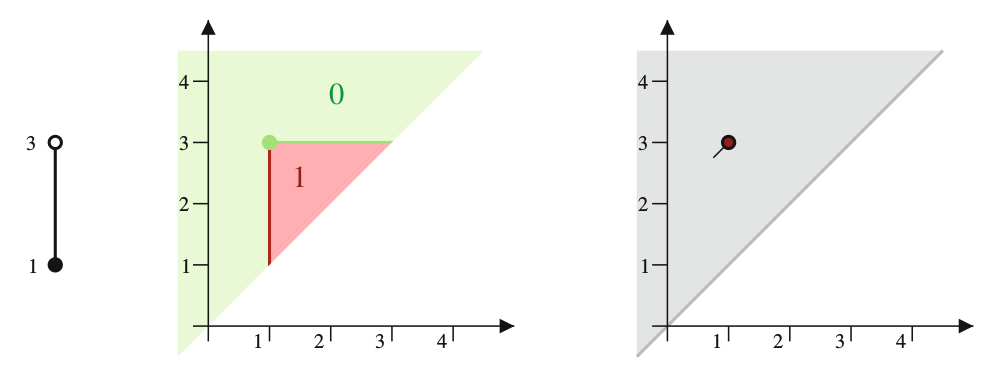
\includegraphics[width=0.7\textwidth]{images/ex_interval_module.png}
    \caption{Representação por intervalo (esquerda), pela função rank (meio) e pelo ponto decorado (direita) do 
            módulo intervalar $\mathbf{k}[1,3) = \mathbf{k}(1^-, 3^-)$.}  
    \label{fig:mod_int}
\end{figure}
Os traços representando a decoração são dados por
\begin{center}
    $(p^-,q^-): $ \rotatebox[origin=c]{225}{$\multimap$}

    $(p^-,q^+): $ \rotatebox[origin=c]{135}{$\multimap$}

    $(p^+,q^-): $ \rotatebox[origin=c]{315}{$\multimap$}

    $(p^+,q^+): $ \rotatebox[origin=c]{45}{$\multimap$}
\end{center}

\subsection{Decomposição em módulos intervalares} 

\begin{defi}
    A \textbf{soma direta} $\mathfrak{W} = \mathfrak{U} \oplus \mathfrak{V}$ de dois módulos
    de persistência $\mathfrak{U}$ e $\mathfrak{V}$ é definida por
    \begin{equation*}
        W_t = U_t \oplus V_t, \quad w^s_t = u_t^s \oplus v^s_t
    \end{equation*}
\end{defi}
Esta definição generaliza-se para somar arbitrárias, tanto finitas como infinitas. Vamos agora definir
a indecomponibilidade de um módulo de persistência.

\begin{defi}
    Um módulo de persistência $\mathfrak{W}$ é indecomponível se dada uma decomposição $\mathfrak{U}
    \oplus \mathfrak{V}$, então $\mathfrak{U} = 0$ ou $\mathfrak{W}$ e $\mathfrak{V} = 0$ ou $
        \mathfrak{W}$.
\end{defi}

Podemos estudar os módulos de persistência através de sua decomposição por módulos intervalares. Dado
uma sequência de intervalos $(J_l \mid l \in L)$,
\begin{equation*}
    \mathfrak{V} \cong \bigoplus_{l \in L} \mathbf{k}^{J_l}.
\end{equation*}
Neste caso, podemos pensar que cada intervalo $J_l$ representa uma propriedade. Esta decomposição acaba
sendo muito importante por este motivo. Mas a questão que fica é: quais módulos são decomponíveis em 
intervalos? E porque decompõe-se em módulos intervalares? 

A resposta para a primeira pergunta é respondida pelo Teorema \ref{teo:crawley}. Já para a segunda questão,
os módulos intervalares são indecomponíveis, como mostramos na Proposição \ref{prop:mod_int}.

\begin{propo}
    Seja $\mathfrak{I} = \mathbf{k}^J_T$ um módulo intervalar sobre $\mathbf{T} \subset \mathbb{R}$. 
    Então $\text{End}(\mathfrak{I}) = \mathbf{k}$. 
\end{propo}
\begin{proof}
    Vamos definir uma função $\Phi$ entre $\text{End}(\mathfrak{I})$ e $\mathbf{k}$ que será um isomorfismo
    de aneis.
    Seja $\Phi \colon \mathbf{k} \to \text{End}(\mathfrak{I})$ definida por 
    \begin{equation*}
        \alpha \mapsto \varphi^{\alpha}
    \end{equation*}
    onde $\varphi^\alpha$ é um endomorfismo de $\mathfrak{I}$ tal que $\varphi_t^{\alpha} \colon I_t 
    \to I_t$ e $\varphi^{\alpha}_t (x) = \alpha x$. É fácil ver que a aplicação é um homomorfismo de anéis.
    Vamos definir a inversa de $\Phi$. Para isso, note primeiro que qualquer endomorfismo de $\mathfrak{I}$
    age como multiplicação por escalar em qualquer $I_t$ não nulo. Precisamos mostrar que dados $s,t$, temos 
    que o escalar definido é o mesmo para ambos os casos:
    \begin{align*}
        \Psi^{-1} \colon & \mathfrak{I} \to \mathbf{k} \\
                         & \varphi \mapsto \alpha,
    \end{align*}
    Vamos mostrar que a aplicação está bem definida.
    
    Primeiro, pela observação acima, dados $s,t$ tais que $I_s, I_t \neq 0$, temos que vale o seguinte
    para $\varphi \in \mathfrak{I}$.
    \begin{align*}
        \varphi_s \colon & \mathbf{k} \to \mathbf{k} \\
                         &     x \mapsto \alpha x 
    \end{align*}
    e 
    \begin{align*}
        \varphi_t \colon & \mathbf{k} \to \mathbf{k} \\
                         &     x \mapsto \beta x 
    \end{align*}
    Precisamos mostrar que $\alpha = \beta$, demonstrando a proposição. Mas isso segue pelo 
    diagrama comutativo dos homomorfismos entre módulos de persistência, como podemos ver na 
    \eqref{eq:diag_prop_end}, assumindo que $s \leq t$. 
    \begin{equation}
        \label{eq:diag_prop_end}
        \begin{tikzcd}
            I_s \arrow{d}[swap]{\varphi_s} \arrow{r}{id} & I_t \arrow{d}{\varphi_t} \\
            I_s \arrow{r}{id}                     & I_t                    
        \end{tikzcd} 
    \end{equation}
    No caso acima temos a identidade entre $I_s$ e $I_t$, já que ambos são $\mathbf{k}$. Logo,
    segue que $\alpha=\beta$, provando a Proposição.
\end{proof}

\begin{propo}\label{prop:mod_int}
    Módulos intervalares são indecomponíveis. 
\end{propo}
\begin{proof}
    Suponha que exista uma decomposição $\mathfrak{I} = \mathfrak{U} \oplus \mathfrak{V}$. Considere agora
    as projeções sob $\mathfrak{U}$ e $\mathfrak{V}$. Ambas são homomorfismos idempotentes. Mas como 
    $\text{End}(\mathfrak{I})$ é isomorfo a $\mathbf{k}$ e os únicos idempotentes de $\mathbf{k}$ são 
    $0$ e $1$, segue que $\mathfrak{I}$ é indecomponível. 
\end{proof}

\begin{teo}{(Krull-Remak-Schmidt-Azumaya)}\label{teo:krull}
    Suponha que um módulo de persistência $\mathbf{T} \subset \mathbb{R}$ pode ser escrito como soma 
    direta de módulos intervalores de duas formas diferentes
    \begin{equation*}
        \mathfrak{V} \cong \bigoplus_{l \in L} \mathbf{k}^{J_l} \cong \bigoplus_{m \in M} \mathbf{k}^{K_m},
    \end{equation*}
    então existe uma bijeção $\sigma \colon L \to M$ tal que $J_l = K_{\sigma(l)}$ para todo $l \in L$. 
\end{teo}
\begin{proof}
    A demonstração segue do Teorema $1$~\cite{Azumaya1950} com a observação de que se $\mathbf{k}^J \cong 
    \mathbf{k}^L$, então $J=K$. Só é necessário verificar uma condição de localidade para aplicarmos o teorema:
    se $\psi, \phi \in \text{End}(\mathfrak{I})$ são não isomorfismos, então $\psi + \phi$ não é isomorfismo. 
    Mas pela proposição anterior, isso segue do fato que a unica aplicação que não é isomorfismo em 
    $\text{End}(\mathfrak{I})$ é a aplicação nula.
\end{proof}

\begin{teo}{(Gabriel, Auslander, Ringel-Tachikawa, Webb, Crawley-Boevey)}\label{teo:crawley}
    Seja $\mathfrak{V}$ um módulo de persistência sobre $\mathbf{T} \subset \mathbb{R}$. Então $\mathfrak{V}$
    pode ser decomposto como um soma direta de módulos intervalares sob as seguintes condições:
    \begin{itemize} 
        \item $\mathbf{T}$ é um conjunto finito;
        \item cada $V_t$ é um espaço vetorial de dimensão finita. 
    \end{itemize}
    Por outro lado, existe um módulo de persistência sob $\mathbb{Z}$ que não admite uma decomposição intervalar. 
\end{teo}  
\begin{proof}
    Detalhes podem ser vistos em \cite{Chazal2016}, página 22, \textbf{Teorema} 2.8.
\end{proof}

Se um módulo de persistência indexado sobre $\mathbb{R}$ pode ser decomposto
\begin{equation*}
    \mathfrak{V} \cong \bigoplus_{l \in L} \mathbf(p_l^*, q_l^*),
\end{equation*}
então o diagrama de persistência decorado é definido pelo multiconjunto
\begin{equation*}
    \text{Dgm} (\mathfrak{V}) = \text{Int}(\mathfrak{V}) = \Set{(p_l^*, q_l^*) | l \in L}
\end{equation*}
e o diagram de persistência não decorado é o multiconjunto
\begin{equation*}
    \text{dgm} (\mathfrak{V}) = \text{int}(\mathfrak{V}) = \Set{(p_l, q_l) | l \in L} - \Delta,
\end{equation*}
onde $\Delta$ é a diagonal no plano.

Note que ambos os diagramas definidos não dependem da escolha da decomposição, devido ao Teorema \ref{teo:krull}. 
Além disso, o diagrama dgm é o diagrama de pontos não decorados e sem a diagonal, sendo encontrado com 
frequência em exemplos práticos de análise de dados. Para a definição da distância bottleneck acaba sendo 
mais importante. 

\subsection{Cálculos com quivers}

Vamos agora definir uma notação para trabalhar com módulos de persistência sobre conjuntos de índices 
finitos. 
Um módulo de persistência $\mathfrak{V}$ sobre um conjunto finito de índices
\begin{equation*}
    \mathbf{T} : \qquad a_1 < \dots < a_n 
\end{equation*} 
da reta real pode ser visto como um diagrama de $n$ espaços vetoriais e $n-1$ aplicações lineares, como
mostrado abaixo
\begin{equation*}
    \mathfrak{V} : \quad V_{a_1} \longrightarrow \dots \longrightarrow V_{a_n}.
\end{equation*}
O diagrama acima é a representação do seguinte \textbf{quiver}:
\begin{equation*}
    \bullet \longrightarrow \bullet \longrightarrow \dots \longrightarrow \bullet
\end{equation*}

Vimos que podemos decompor alguns módulos de persistência em módulos intervalares. Para estes podemos representa-los 
com quivers da seguinte forma. 
\begin{ex}
    Seja $a < b < c$. Existem $6$ módulos intervalares diferentes sobre este intervalo.
\begin{equation*} 
    \begin{matrix}
        \mathbf{k}[a,a] = \qon{a} \qem \qoff{b} \qem \qoff{c} & \mathbf{k}[a,b] = \qon{a} \qem \qon{b} \qem \qoff{c}& 
                            \mathbf{k}[a,c] = \qon{a} \qem \qoff{b} \qem \qon{c}\\
        \mathbf{k}[b,b] = \qoff{a} \qem \qon{b} \qem \qoff{c}& \mathbf{k}[b,c] = \qoff{a} \qem \qon{b} \qem \qon{c}& \\
        \mathbf{k}[c,c] = \qoff{a} \qem \qoff{b} \qem \qon{c}& & & 
    \end{matrix}
\end{equation*}
\end{ex}

Os círculos $\bullet$ representam uma cópia do espaço vetorial $\mathbf{k}$ unidimensional. O círculo $\circ$ representa o 
espaço vetorial nulo. A aplicação linear entre dois $\bullet$ é a identidade e qualquer aplicação contendo $\circ$ é a
nula.

Esta notação pode ser usada para representar a multiplicidade dos módulos intervalares da decomposição
de um módulo de persistência sobre um conjunto de índices finito, essa quando existe. Seja $\mathfrak{V}$
um módulo de persistência sobre o conjunto $\mathbf{T} = \Set{a_1, \dots, a_n}$. Definimos a multiplicidade
de $[a_i, a_j] \subseteq \mathbf{T}$ em $\mathfrak{V}_{\mathbf{T}}$ como o número de cópias do módulo
$\mathbf{k}[a_i,a_j]$ na decomposição de $\mathfrak{V}_{\mathbf{T}}$. 

\begin{ex}
    Seja $\mathfrak{V}$ módulo de persistência sobre $\mathbf{T} = \Set{a,b,c}$. Escrevemos
    \begin{equation*}
        \innerproduct{[b,c] \mid \mathfrak{V}_{\mathbf{T}}} \text{ ou } \innerproduct{\qoff{a} \qem \qon{b} 
        \qem \qon{c} \mid \mathfrak{V}}
    \end{equation*}
    para representar a multiplicidade de $\qoff{a} \qem \qon{b} \qem \qon{c}$ no seguinte módulo de $3$ termos
    \begin{equation*}
        \mathfrak{V} : \quad V_{a_1} \longrightarrow \dots \longrightarrow V_{a_n}.
    \end{equation*}
\end{ex}

\begin{ex}
    Considere o módulo com dois espaços vetoriais e uma única aplicação linear $\mathfrak{V} : \quad 
    V_a \xrightarrow{\mu} V_b$. Então os invariantes de $\mu$ são
    \begin{align*}
        \text{rank}(\mu)       & = \innerproduct{\qon{a} \qem \qon{b} \mid \mathfrak{V}}, \\
        \text{nulidade}(\mu)   & = \innerproduct{\qon{a} \qem \qoff{b} \mid \mathfrak{V}}, \\
        \text{conulidade}(\mu) & = \innerproduct{\qoff{a} \qem \qon{b} \mid \mathfrak{V}}.
    \end{align*}
    Basta notar que para $V_a, V_b$ espaços de dimensão finita, existe uma decomposição das suas bases 
    \begin{equation*}
        e_1, \dots, e_r, f_1, \dots, f_n \text{   e   } g_1, \dots, g_r, h_1, \dots, h_m
    \end{equation*}
    tais que $\mu(e_i) = g_i$, $\mu(f_j) = 0$ para todo $i,j$. Assim, os espaços vetoriais unidimensionais
    gerados pelos elementos das bases geram uma decomposição do módulo $\mathfrak{V}$ nos seguintes intervalos
    \[\begin{array}{ccccc}
        (&\text{span}(e_i) & \rightarrow &\text{span}(g_i)&) \\
        (&\text{span}(f_j) & \rightarrow &0               &) \\
        (& 0               & \rightarrow &\text{span}(h_k)&)
    \end{array}\]
    que são isomorfos respectivamente à $\qon{a} \qem \qon{b}$, $\qon{a} \qem \qoff{b}$ e 
    $\qoff{a} \qem \qon{b}$. 
\end{ex}

\begin{propo}
    Suponha que podemos decompor um módulo de persistência $\mathfrak{V}$ como uma soma direta
    \begin{equation*}
        \mathfrak{V} = \bigoplus_{l\in L} \mathfrak{V}^l,
    \end{equation*}
    então 
    \begin{equation*}
        \langle [a_i, a_j] \mid \mathfrak{V}_{\mathbf{T}} \rangle = \sum_{l\in L} \langle [a_i, a_j] 
        \mid \mathfrak{V}_{\mathbf{T}}^l \rangle
    \end{equation*}
    para qualquer conjunto de índices $\mathbf{T} = \Set{a_1, \dots, a_n}$ e intervalos $[a_i, a_j] \subseteq \mathbf{T}$.
\end{propo}
\begin{proof}
    Segue do fato que a decomposição intervalar de $\mathfrak{V}_{\mathbf{T}}$ é a soma direta das decomposições intervalares 
    de cada $\mathfrak{V}^l_{\mathbf{T}}$ para todo $l \in L$. 
\end{proof}

\begin{propo}{(Princípio da restrição)}
    Sejam $\mathbf{S}, \mathbf{T}$ conjuntos de índices com $\mathbf{S} \subset \mathbf{T}$. Então
    \begin{equation*}
        \langle I \mid \mathfrak{V}_{\mathbf{S}} \rangle = 
        \sum_{J} \langle J \mid \mathfrak{V}_{J} \rangle,
    \end{equation*}
    onde a soma é sobre todos os intervalos $J \subseteq \mathbf{T}$ que se restringe a 
    $I$ sobre $\mathbf{S}$. 
\end{propo}
\begin{proof}   
    Tome uma decomposição intervalar arbitrária de $\mathfrak{V}_{\mathbf{T}}$. Então uma decomposição
    intervalar é induzida em $\mathfrak{V}_{\mathbf{S}}$. Note agora que para $I \subseteq \mathbf{S}$,
    temos diversos intervalos $J \subseteq \mathbf{T}$ tais que $J \cap \mathbf{S} = I$. Devido a 
    linearidade da soma direta, temos que os intervalos de $\mathfrak{V}_{\mathbf{S}}$ do tipo $I$ 
    são os intervalos de $\mathfrak{V}_{\mathbf{T}}$ do tipo $J$ acima. 
\end{proof}
\begin{ex}
    Seja $a < p < b < q < c$. Então temos os seguintes exemplos para os conjuntos de índices:
    \begin{itemize}
        \item $\mathbf{T}_1 = \Set{a,b,q,c}$, $S_1=\Set{a,b,c}$, $I_1=[b,c]$.
        \begin{equation*}
            \innerproduct{\qoff{a} \qem \qno \qem \qon{b} \qem \qno \qem \qon{c}} =
            \innerproduct{\qoff{a} \qem \qno \qem \qon{b} \qem \qon{q} \qem \qon{c}} 
        \end{equation*}
        \item $\mathbf{T}_2 = \Set{a,p,b,c}$, $S_2=\Set{a,b,c}$, $I_2=[b,c]$.
        \begin{equation*}
            \innerproduct{\qoff{a} \qem \qno \qem \qon{b} \qem \qno \qem \qon{c}} =
            \innerproduct{\qoff{a} \qem \qoff{p} \qem \qon{b} \qem \qno \qem \qon{c}}
            + \innerproduct{\qoff{a} \qem \qon{p} \qem \qon{b} \qem \qno \qem \qon{c}} 
        \end{equation*}
        \item $\mathbf{T}_3 = \Set{a,b,q,c}$, $S_2=\Set{a,b,c}$, $I_2=[c,c]$.
        \begin{equation*}
            \innerproduct{\qoff{a} \qem \qno \qem \qoff{b} \qem \qno \qem \qon{c}} =
            \innerproduct{\qoff{a} \qem \qno \qem \qoff{b} \qem \qoff{q} \qem \qon{c}}
            + \innerproduct{\qoff{a} \qem \qno \qem \qoff{b} \qem \qon{q} \qem \qon{c}} 
        \end{equation*}
         
    \end{itemize}
\end{ex}
\section{Medidas retangulares}

\subsection{A medida de persistência}

\subsection{r-medidas abstratas}

\subsection{Equivalência de medidas e diagramas}

\section{Comportamento de módulos e exemplos}

\section{\textit{Interleaving}} 

\section{O teorema de isometria}
